\chapter{Knowledge injection}

\begin{remark}
    ML models exploit implicit knowledge from the data. Explicit knowledge (e.g., rules-of-thumb, known correlations and causal factors, laws of physics, \dots) is instead not used.
\end{remark}



\section{Approaches}


\subsection{Generative approach}

\begin{description}
    \item[Generative approach] \marginnote{Generative approach}
        Use symbolic knowledge to create training samples that are used to train a model.

        \begin{remark}
            This approach does not let the model exploit explicit knowledge and might be inefficient.
        \end{remark}
\end{description}



\subsection{Lagrangian approaches}

\begin{description}
    \item[Knowledge as constraint] 
        Use hard or soft constraints to inject knowledge.

        \begin{example}[RUL estimation]
            For RUL estimation, a simple explicit knowledge is that RUL decreases by 1 unit each time step. Formally, given two pairs of examples $(x_i, y_i)$ and $(x_j, y_j)$, it holds that:
            \[ y_i - y_j = j - i \quad \forall i,j = 1, \dots, m \text{ with } c_i = c_j \]
            where $c_k$ indicates the machine of the $k$-th sample.
            Given a model $f$, it can be constrained as follows:
            \[ f(x_i; \theta) - f(x_j; \theta) \approx j - i \]
            Its training problem becomes:
            \[ \arg\min_\theta \mathcal{L}(y, f(x; \theta)) \text{ subj. to } f(x_i; \theta) - f(x_j; \theta) \approx j - i \]
        \end{example}


    \item[Lagrangian approaches] \marginnote{Lagrangian approaches}
        Given:
        \begin{itemize}
            \item A training problem: $\arg\min_\theta \{ \mathcal{L}(\hat{y}) \mid \hat{y} = f(x; \theta) \}$,
            \item Some constraints defined as an inequality on a vector function $\vec{g}(\hat{y}) \leq 0$ with $\vec{g}(\hat{y}) = \{ g_k(\hat{y}) \}_{k=1}^{m}$.
        \end{itemize}

        \begin{description}
            \item[Naive formulation] 
                The constraints can be formulated as a loss penalty as follows:
                \[ \mathcal{L}(\theta, \vec{\lambda}) = \mathcal{L}(\hat{y}) + \vec{\lambda}^T \vec{g}(\hat{y}) \]
                where $\vec{\lambda}$ is a vector of multipliers (Lagrangian multipliers).

                \begin{remark}
                    $g_k(\hat{y}) = 0$ and $g_k(\hat{y}) \leq 0$ both satisfy the constraint. However, if $g_k(\hat{y})$ goes below $0$, it becomes an unwanted reward.

                    In classical Lagrangian theory, this is solved by changing the sign of $\lambda_k$. However, this works by assuming convexity and requires optimizing for $\vec{\lambda}$.
                \end{remark}

            \item[Clipped formulation] 
                The constraints can be formulated as a loss penalty as follows:
                \[ \mathcal{L}(\theta, \vec{\lambda}) = \mathcal{L}(\hat{y}) + \vec{\lambda}^T \max\{ 0, \vec{g}(\hat{y}) \} \]
                with $\vec{\lambda} \geq 0$.

                \begin{remark}
                    An equality constraint $g_k(\hat{y}) = 0$ can be formulated as:
                    \[ 
                        g_k(\hat{y}) \leq 0 \land -g_k(\hat{y}) \leq 0  
                    \]
                    In penalty terms, it becomes:
                    \[
                        \lambda_k' \max \{ 0, g_k(\hat{y}) \} + \lambda_k'' \max \{ 0, -g_k(\hat{y}) \} = \lambda_k | g_k(\hat{y}) |
                    \]
                    where $\lambda_k = \lambda_k' + \lambda_k''$.

                    An alternative formulation is also:
                    \[ \vec{\lambda}^T \vec{g}(\hat{y})^2 \]
                    which is due to normal distribution properties.
                \end{remark}
        \end{description}

        \begin{remark}
            Lagrangian approaches usually work with differentiable constraints, but it is not strictly required. However, differentiability is needed for training with gradient descent.
        \end{remark}

        \begin{description}
            \item[Multipliers calibration (maximal accuracy)]
                Consider constraints in a soft manner. The penalty can be considered as a regularizer and $\vec{\lambda}$ can be considered as a hyperparameter and optimized through hyperparameter tuning.

                \begin{remark}
                    This approach is viable when sufficient data is available.
                \end{remark}

            \item[Multipliers calibration (constraints satisfaction)]
                Consider constraints in a hard manner.

                \begin{description}
                    \item[Naive approach] 
                        Use a large $\vec{\lambda}$.
                        \begin{remark}
                            This approach leads to numerical instability and disproportional gradients.
                        \end{remark}

                \item[Dual ascent] \marginnote{Dual ascent}
                    \begin{remark}
                        The loss with the constraint penalty is differentiable in $\vec{\lambda}$:
                        \[ \nabla_\lambda \mathcal{L}(\theta, \vec{\lambda}) = \max \{ 0, \vec{g}(f(x, \theta)) \} \]
                        where:
                        \begin{itemize}
                            \item If the constraint is satisfied, the partial derivative is $0$.
                            \item If the constraint is violated, the partial derivative is equal to the violation.
                        \end{itemize}
                    \end{remark}

                    Alternate gradient descent and ascent. The method works as follows:
                    \begin{enumerate}
                        \item Initialize the multipliers $\vec{\lambda}^{(0)} = 0$.
                        \item Until a stop condition is met:
                        \begin{enumerate}
                            \item Obtain $\vec{\lambda}^{(k)}$ via gradient ascent with $\nabla_\vec{\lambda} \mathcal{L}(\theta^{(k-1)}, \vec{\lambda})$.
                            \item Obtain $\theta^{(k)}$ via gradient descent with $\nabla_\theta \mathcal{L}(\theta, \vec{\lambda}^{(k)})$.
                        \end{enumerate}
                    \end{enumerate}
                \end{description}
        \end{description}

        \begin{remark}
            Lagrangian approaches are enforced at training time. Constraints might be violated at test time.
        \end{remark}

        \begin{example}[RUL estimation]
            The constraint:
            \[ f(x_i; \theta) - f(x_j; \theta) \approx j - i \]
            can be formulated as the following penalty:
            \[ \lambda \sum_{\substack{i,j=1, \dots, m\\c_i = c_j}} (f(x_i; \theta) - f(x_j; \theta) - (j-i))^2 \]
            where $\lambda$ is the same for all pairs for simplicity.
            Moreover, to avoid redundances, it is reasonable to only consider consecutive time steps (denoted as $i \prec j$):
            \[ \lambda \sum_{\substack{i \prec j\\c_i = c_j}} (f(x_i; \theta) - f(x_j; \theta) - (j-i))^2 \]

            \indenttbox
            \begin{remark}
                With batches, consecutivity refers to the closest available time step  of the same machine in the same batch.

                It is also necessary to sample batches in such a way that at least two time steps of the same machine are considered (otherwise the gradient step would be wasted).
            \end{remark}

            \begin{figure}[H]
                \centering
                \begin{subfigure}{0.6\linewidth}
                    \centering
                    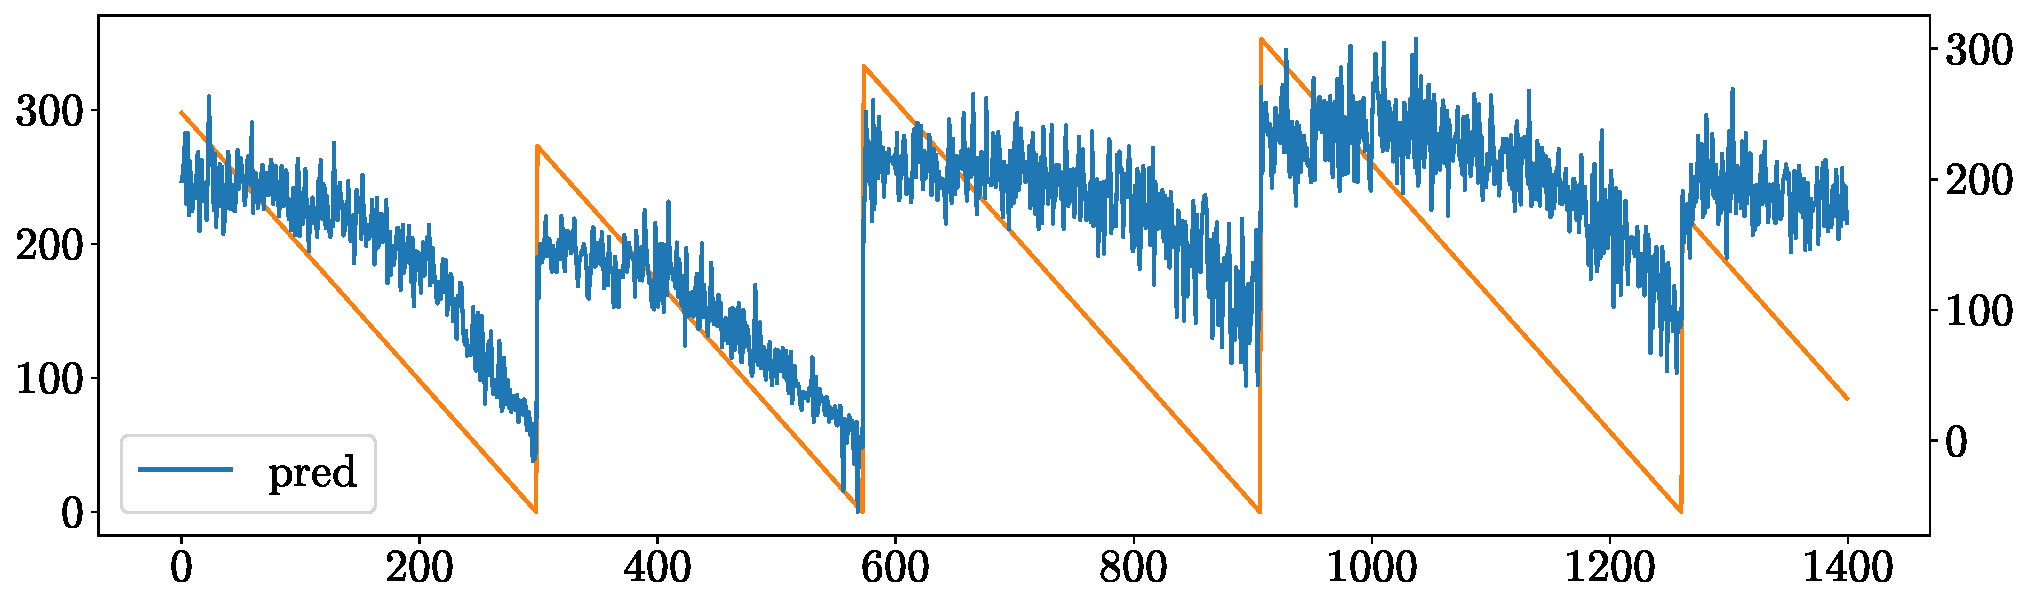
\includegraphics[width=\linewidth]{./img/_rul_pre_lagrangian.pdf}
                    \caption{Results without knowledge injection}
                \end{subfigure}
                \begin{subfigure}{0.6\linewidth}
                    \centering
                    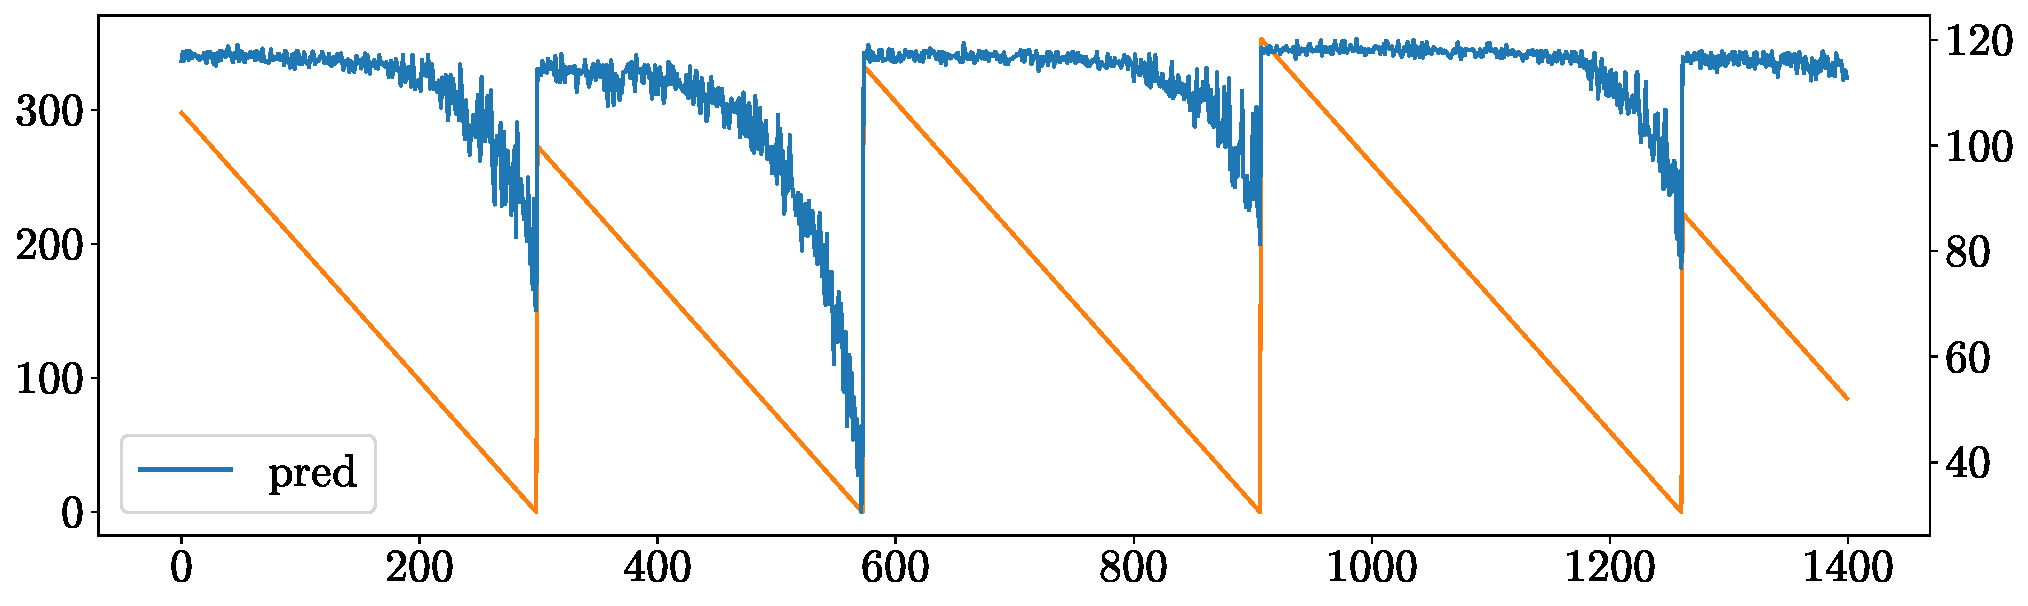
\includegraphics[width=\linewidth]{./img/_rul_lagrangian.pdf}
                    \caption{Results with knowledge injection (note that the scales are off)}
                \end{subfigure}
            \end{figure}
        \end{example}
\end{description}


\subsection{Ordinary differential equations learning}

\begin{description}
    \item[Ordinary differential equation (ODE)] \marginnote{Ordinary differential equation (ODE)}
        Equation defined as:
        \[ \dot{y} = f(y, t) \]
        where $\dot{y}$ is the rate of change and $y$ is the state variable defined as a function of (usually) time $t$ (i.e., $y(t)$ is the state at time $t$).

        \begin{remark}
            This class of differential equations can be seen as a transition system with continuous steps.
        \end{remark}

        \begin{remark}
            ODEs are useful to represent physics knowledge.
        \end{remark}

    \item[Initial value problem] \marginnote{Initial value problem}
        Given an ODE $\dot{y} = f(y, t)$ and an initial state $y(0) = y_0$, determine how the states unfold (i.e., run a simulation).

        \begin{description}
            \item[Euler method] \marginnote{Euler method}
                Solve an initial value problem by discretizing time and computing the transition function at time $t$ as:
                \[ y_k = y_{k-1} + (t_k - t_{k-1}) f(y_{k-1}, t_{k-1}) \]
                It is assumed that the solution is piece-wise linear (i.e., linearity between two consecutive states).

                \begin{figure}[H]
                    \centering
                    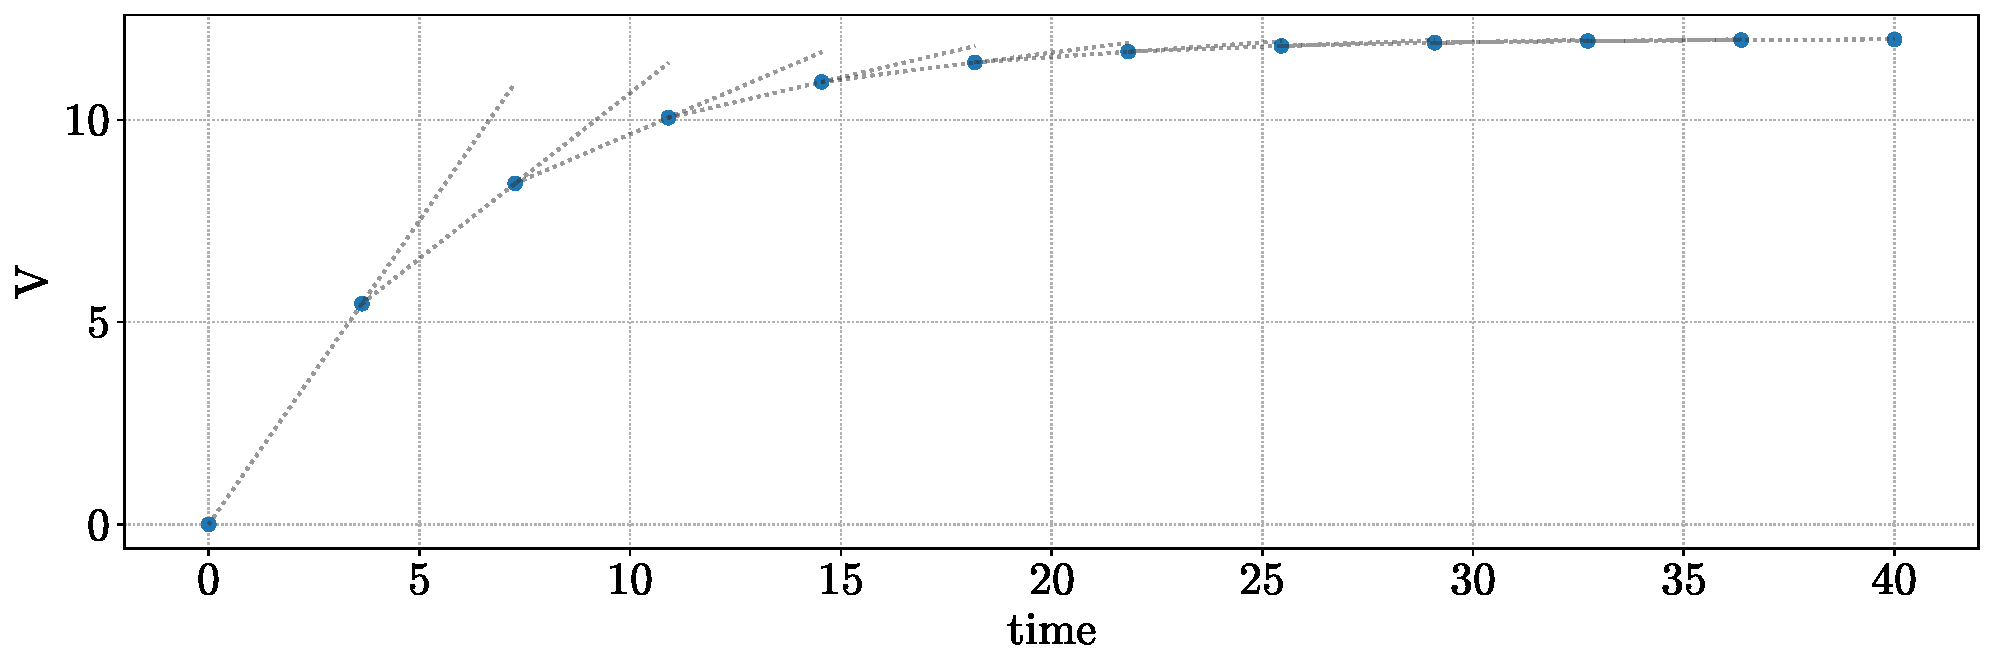
\includegraphics[width=0.7\linewidth]{./img/_rc_euler.pdf}
                \end{figure}

                \begin{remark}
                    Euler method does not perform well in terms of accuracy. There are variants with better performance.
                \end{remark}
        \end{description}

    \item[Learning ODE] \marginnote{Learning ODE}
        Estimate the parameters of an ODE from the data. The training problem is defined as:
        \[ \arg\min_\theta \{ \mathcal{L}(\hat{y}(t), y) \mid \dot{\hat{y}} = f(\hat{y}, t; \theta) \land \hat{y}(0) = y_0 \} \]

        A possible approach is to discretize time and optimize on the relaxed problem. The steps are:
        \begin{enumerate}
            \item Solve the initial value problem using a numerical method (e.g., Euler).
            \item Compute the loss $\mathcal{L}$ and optimize over $\theta$.
        \end{enumerate}

        \begin{remark}
            This path can be taken if the integration steps are differentiable. Euler method is differentiable.
        \end{remark}

        \begin{description}
            \item[Architecture]
                The method can be implemented in an RNN fashion with the Euler method encoded into a repeated layer. At each step, the networks takes as input the state and the time variable, and estimates a new state.

                \begin{figure}[H]
                    \centering
                    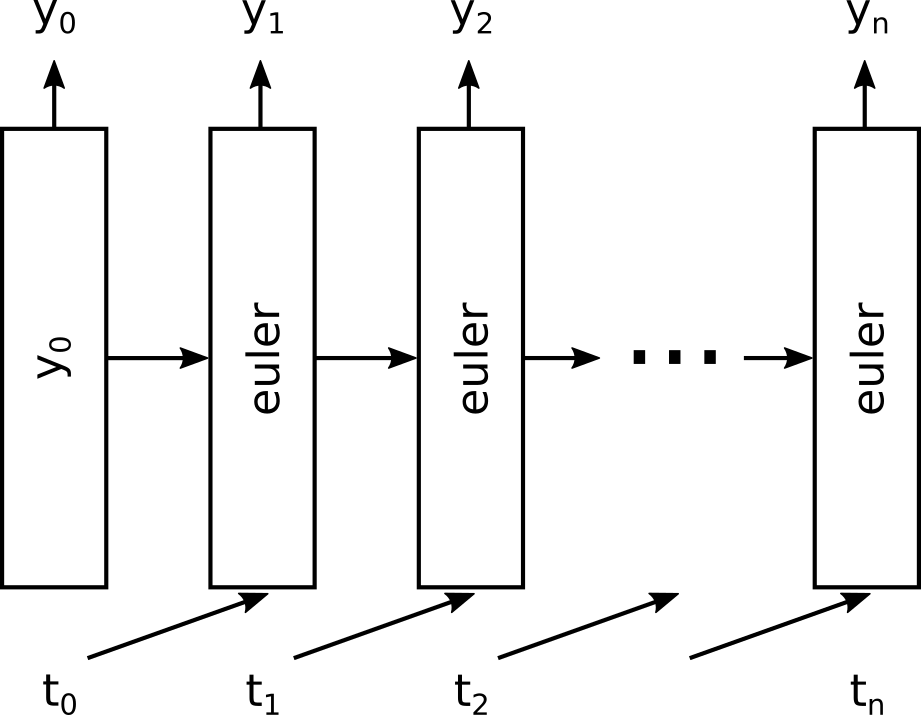
\includegraphics[width=0.3\linewidth]{./img/rc_ode_learning.png}
                \end{figure}
        \end{description}

        \begin{remark}
            This approach is slow to converge and is not very accurate.
        \end{remark}

        \begin{example}
            Consider an RC circuit with a voltage source $V_S$, a capacitor $C$, and a resistor $R$.
            \begin{figure}[H]
                \centering
                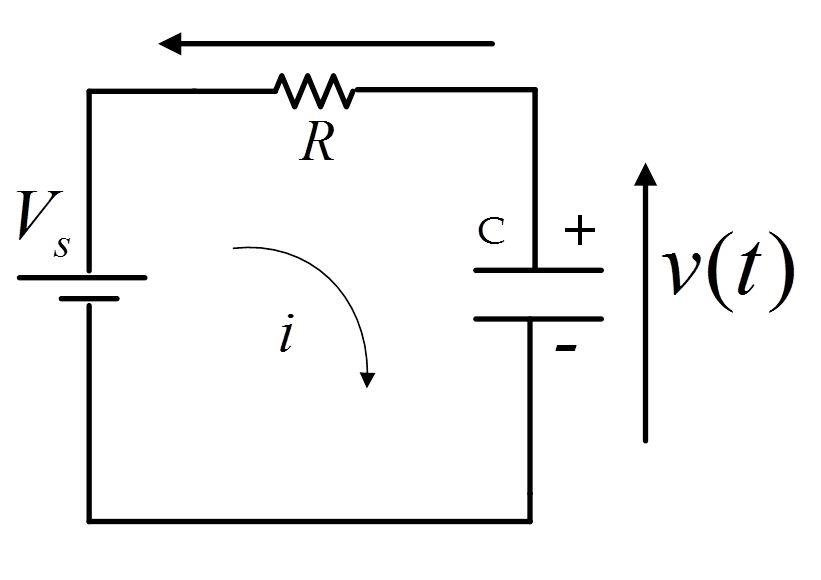
\includegraphics[width=0.23\linewidth]{./img/rc_circuit.png}
            \end{figure}
            Its dynamic behavior is described by the ODE:
            \[ \dot{V} = \frac{1}{\tau}(V_S - V) \]
            where $\tau = RC$.

            Assume that we have a dataset of the ground-truth voltage $y$ at each time step and we want to find the parameters $V_S$ and $\tau$ of the ODE. The problem is defined as:
            \[ \arg\min_{V_S, \tau} \mathcal{L}(\hat{y}(t), y) \text{ subj. to } \dot{\hat{y}} = \frac{1}{\tau} (V_S - \hat{y}) \land \hat{y}(0) = y_0 \]

            A layer of the neural network estimates $V_S$ and $\tau$. The time steps are passed through the network and all the predicted voltages are used to compute the loss.

            Note that $V_S$ and $\tau$ must be positive values. We can use the same trick as in \Cref{sec:arrivals_neuroprob} by using $\exp\log$ with a scaling factor to start with a reasonable guess.
        \end{example}
\end{description}